%%%%%%%%%%%%%%%%%%%%%%%%%%%%%%%%%%%%%%%%%
%
% Funkcionalna verifikacija hardvera
% 
%%%%%%%%%%%%%%%%%%%%%%%%%%%%%%%%%%%%%%%%%

Vežba 11 je posvećena prikupljanju pokrivenosti. Dat je kratak pregled tipova
pokrivenosti, prednosti i mana i objašnjen način implementacije koristeći
SystemVerilog. Pokazane su i mogućnosti alata u pogledu prikupljanja
pokrivenosti.

%========================================================================================
% Section
%========================================================================================

\section{Uvod}

Jedan od težih zadataka u procesu verifikacije je odlučiti kada je verifikacija
završena. Da bi smo došli do tog zaključka mora se odgovoriti na dva pitanja: da
li su sve osobine dizajna, koje su identifikovane u verifikacionom planu,
verifikovane? I da li postoje delovi koda u dizajnu koji se nikad nisu
koristili? Da bi smo dali odgovore na ova pitanja uvodi se nova metrika -
pokrivenost (engl. \emph{coverage}). Sa porastom veličine i kompleksnosti
sistema, merenje pokrivenosti je postalo neophodan deo svakog verifikacionog
ciklusa. Pored zaključka o kraju verifikacije, pokrivenost pomaže i pri analizi
toka verifikacije dajući odgovore na pitanja nalik: kada je testirana jedna
osobina, da li se u isto vreme proverila i neka druga osobina? Da li je proces
uporen iz nekog razloga? Da li je moguće smanjiti broj testova kako bi se ubrzao
proces, a da se i dalje sve potrebne osobine verifikuju?\\

Ukratko, \emph{coverage} je metrika koja se koristi za merenje progresa i
završetka verifikacije. Daje informacije o tome kada se neki deo dizajna
aktivirao tokom simulacije i, što je možda i važnije, da li postoje delovi
dizajna koji nikad nisu bili aktivirani. Sa ovim informacijama je moguće
podesiti stimulus kako bi ostvarili ciljeve.\\

Dve najčešće korišćene \emph{coverage} metrike su:

\begin{itemize}
\item Strukturna pokrivenost (engl. \emph{code coverage}) - implicitna
\item Funkcionalna pokrivenost (engl. \emph{functional coverage}) - eksplicitna
\end{itemize}

Pojedinačne metrike nisu dovoljne da bi smo došli do odgovarajućih zaključaka.
Npr. moguće je ostvariti 100\% pokrivenosti koda, a da neke osobine uopšte nisu
verifikovane. Takođe je moguće ostvariti 100\% funkcionalne pokrivenosti, a
manji procenat pokrivenosti koda. Zato se uvek koriste obe metrike, uz detaljno
razrađen plan o prikupljanju pokrivenosti.\\

U nastavku vežbe objašnjene su obe metrike, sa posebnim akcentom na
funkcionalnoj pokrivenosti.

%========================================================================================
% Section
%========================================================================================

\section{Strukturna pokrivenost}

Strukturna pokrivenost ili pokrivenost koda daje informacije o stepenu
aktivacije sors koda tokom verifikacije čime se omogućava praćenje struktura
koje se nikad ne aktiviraju. Glavna prednost ove metrike je što je implicitna
odnosno kreiranje modela je automatsko. Za korišćenje pokrivenosti koda nije
potrebno dodavati poseban kod i ne zahteva poseban pristup tokom verifikacije.\\

Mana ovog tipa pokrivenosti je što je moguće imati 100\% pokrivenosti, a da i
dalje postoje greške u dizajnu. Npr. stimulus je aktivirao liniju koja sadrži
grešku, ali efekti nisu propagirani dovoljno da bi je odgovarajuće provere
uhvatile. Drugo ograničenje je što ne daje indikacije o samoj funkcionalnosti.
Npr. moguće je da postoji deo funkcionalnosti DUT-a koji nikad nije verifikovan,
a možda nije čak ni implementiran. Iako bi tada imali 100\% pokrivenosti koda,
proces verifikacije ne bi bio uspešan. I pored ovih problema, zbog automatskog
prikupljanja, pokrivenost koda se jako puno koristi i daje dobre indikacije o
toku same verifikacije.\\

Postoji više tipova strukturne pokrivenosti. U nastavku su ukratno opisane. Za
detalje pogledati odgovarajuće predavanje.

\begin{itemize}
\item \emph{Toggle coverage} - meri koliko puta je svaki bit registra ili
  signala promenio vrednost. Analiza svih ovih podataka može biti redudantna,
  ali je i dalje korisna u nekim situacijama npr. kod povezanosti dva IP bloka
\item \emph{Line coverage} - meri koje linije koda su aktivirane tokom
  simulacije i koliko puta. Ova metrika često okriva da postoji deo koda koji se
  jako retko aktivira zbog manja stimulusa ili da postoji deo koda koji se nikad
  ne koristi npr. zbog konfiguracije IP-a
\item \emph{Statement coverage} - meri koje naredbe su aktivirane i koliko puta.
  Često je korisnije od merenja linija jer jedna naredba može sadržati više
  linija koda, ali i više naredbi može postojati u jednoj liniji
\item \emph{Block coverage} - varijacija \emph{statement coverage}-a koja meri
  da li se blok koda izvršio. Blok čine naredbe unutar uslovnih naredbi ili
  unutar proceduralne definicije. Ideja je da kada se dođe do određenog bloka,
  sve naredbe unutar njega će biti izvršene
\item \emph{Branch coverage} - meri da li su uslovi unutar kontrolnih strukura
  (\emph{if}, \emph{case}, \emph{while}, \emph{for}, \emph{repeat}, ...)
  evaluirane i kao tačne i kao netačne.
\item \emph{Expression coverage} - meri da li je svaki operand unutar uslova
  evaluiran i kao tačan i kao netačan
\item \emph{Finite-state machine coverage} - pošto je alat u mogućnosti da
  identifikuje FSM u RTL-u, moguće je prikupljati informacije o pokrivenosti,
  npr. koliko puta se ušlo u svako stanje ili da li su svi prelazi viđeni
\end{itemize}

Pogledati četvro poglavlje za informacije o alatu i kako doći do podataka o ovom
tipu pokrivenosti.

%========================================================================================
% Section
%========================================================================================

\section{Funkcionalna pokrivenost}

Cilj funkcionalne verifikacije je utvrditi da li dizajn implementira sve osobine
i funkcioniše na način opisan u funkcionalnoj specifikaciji. Međutim do
zaključka o tome da li je neka funkcionalnost stvarno implemntirana i da li je
verifikovana, ne možemo doći na osnovu praćenja pokrivenosti koda. Zbog toga se
uvodi nova, eksplicitna metrika - funkcionalna pokrivenost. Cilj ove metrike je
merenje progresa verifikacije u odnosu na funkcionalne zahteve dizajna.\\

Jedan od problema korićenja \emph{constrained-random} pristupa generisanja
stimulusa je što ne znamo tačno koje funkcionalnosti se verifikuju (šta je tačno
dovedeno na ulaz DUT-a) bez da ručno analiziramo \emph{waveform}-e tokom
simulacije. Međutim, praćenje funkcionalne pokrivenosti nam omogućava upravo
ovo - određivanje funkcionalnosti koje su verifikovane bez vizuelne analize
samih signala.\\

Mane ove metrike su što, pošto nije implicitna, ne može biti automatski
implementirana. Implementacija dobrog modela pokrivenosti zahteva dosta vremena
pošto je potrebno prvenstveno napraviti dobar plan, identifikovati sve osobine
od interesa i odrediti način na koji će se prikupljati podaci o pokrivenosti.
Nakon toga, potrebno je izvršiti samu implementaciju u okruženju.\\

U SystemVerilog jeziku postoje dve glavne konstrukcije pomoću kojih je moguće
implementirati ovu metriku:

\begin{itemize}
\item \emph{Cover groups} - obuhvata prikupljanje vrednosti različitih
  promenljivih. Ove vrednosti se prikupljaju bilo nadgledanjem interfejsa,
  registara, kontrolnih signala... Vrednosti koje se mere se uzimaju u jednom
  vremenskom trenutku.
\item \emph{Cover properties} - opisuje temporalne osobine između sekvenci
  različitih događaja. Najčešće se koriste za proveru \emph{handshake} sekvenci
  u nekom protokolu (npr. posle \emph{req} sledi \emph{ack} i sl.)
\end{itemize}

Na ovom kursu ćemo se zadržati na modelovanju grupa, što je i najčešći način
impementacije modela pokrivenosti. Za informacije o \emph{cover propety}
zainteresovani studenti neka pogledaju odgovarajuće poglavlje u
``Cookbook''-u.\\

U nastavku je dat jednostavan primer sakupljanja funkcionalne pokrivenosti za
memoriju. U primeru postoji jedna grupa čiji se uzorak uzima na svakoj rastućoj
ivici en signala i uzimaju se vrednosti adrese (u tri opsega), parnosti (za
parnu i neparnu) i \emph{rw} (čitanje ili upis). Nakon simulacije ovog koda,
možemo videti informacije o funkcionalnoj pokrivenosti - koje vrednosti adresa
su viđene, koji tip parnosti i da li se vršio upis ili čitanje. Deo izveštaja
je takođe prikazan. Iz njega možemo zaključiti da su viđene adrese iz donjeg
opsega, pri čemu je viđena samo \emph{read} operacija uz \emph{even} parnost.

\lstinputlisting[caption=Primer sakupljanja funkcionalne pokrivenosti, label=lst:simple_coverage]{code/v11_simple_coverage.sv}

\begin{figure}[h!]
  \center
  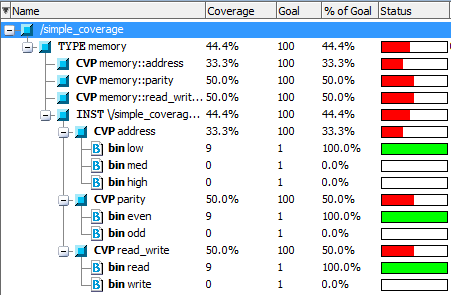
\includegraphics[width=100mm, scale=0.5]{img/v11_simple_coverage.png}
  \caption{Primer sakupljanja funkcionalne pokrivenosti}
  \label{fig:simple_coverage}
\end{figure}

U nastavku je dat detaljan opis strukture grupe i njenih mogućnosti.

% ----------------------------------------------------------------------------------------

\subsection{Implementacija}

\emph{Covergroup} konstrukcija je tip definisan od strane korisnika. Samo jednom
se definiše, a moguće je instancirati ih više puta. Ima dosta sličnosti sa
klasama. Jedom kada se definiše, instance se kreiraju pozivanjem \emph{new}.
Sama grupa se može definisati u \emph{package}-u, modulu, program, interfesju
ili klasi.\\

Grupa se definiše korišćenjem \emph{covergroup} i \emph{endgroup} ključnih reči,
a instancira pozivom \emph{new}. Npr.:

\begin{lstlisting}
covergroup cg_example
  // ...
endgroup
cg_example cg = new();
\end{lstlisting}

Napomena: grupa za pokrivenost mora biti instancirana u klasama kako bi
sakupljala podatke. Česta greška je zaboraviti poziv \emph{new}. U tom slučaju
neće biti prijavljena greška i grupa se neće pojavljivati u finalnom
izveštaju.\\

U UVM okruženju, grupe za praćenje pokrivenosti se uglavnom definišu i kreiraju
u odgovarajućim komponentama i na odgovarajućem hijerarhijskom nivou. Uglavnom
su sadržane u odgovarajućim komponentama za analizu: monitorima,
\emph{scoreboard}-u ili posebnim \emph{coverage collector} komponentama čija je
jedina uloga sakupljanje funkcionalne pokrivenosti.\\

\emph{Covergroup}-a može sadržati:

\begin{itemize}
\item Događaj - definiše kada se uzima uzorak. Ukoliko se izostavi korisnik
  mora eksplicitno pozvati metodu
\item tačke pokrivenosti (engl. \emph{coverpoint})- može biti promenljiva ili
  izraz
\item \emph{Cross coverage} - između dve ili više tačaka pokrivenosti
\item Opcije - kontrolišu ponašanje grupe
\item Opcione formalne argumente
\end{itemize}

Svi navedeni konstrukti su detaljnije objašnjeni u narednim poglavljima.

\subsubsection{\emph{Trigerovanje}}

Osim definisanja strukture grupe, potrebno je i odlučiti u kom trenutku će se
uzimati uzorci tj. kada su podaci spremni za semplovanje. Postoji više načina na
koje je ovo moguće specificirati. U nastavku su objašnjeni najčešće korišćeni.\\

Prilikom definisanja grupe, moguće je i definisati događaj na kojem će se
uzimati uzorci. Npr:

\begin{lstlisting}
event e1;
covergroup cg_example @(e1);
  coverpoint x;
endgroup
// ...
cg_example cg = new();
\end{lstlisting}

U ovom slučaju podaci se prikupljaju prilikom svakog događaja \emph{e1}.\\

Drugi način trigerovanja grupe je eksplicitnim pozivanjem funkcije
\emph{sample()}. Npr:

\begin{lstlisting}
covergroup cg_example;
  coverpoint x;
endgroup
// ...
cg_example cg = new();
// ...
cg.sample();
// ...
\end{lstlisting}

Pozivanje funkcije \emph{sample} nad instancom se može obaviti u bilo kom
trenutku.

\subsubsection{Sakupljanje podataka}

Informacije o pokrivenosti se sakupljaju korišćenjem tačaka pokrivenosti (engl.
\emph{coverpoint}). Oni zapravo predstavljaju promenljivu ili izraz koji služi
za prosleđivanje vrednosti od interesa. Kada se tačka definiše, kreira se
određeni broj \emph{bin}-ova koji služe za praćenje samih vrednosti i koliko
puta su određene vrednosti viđene tokom simulacije. \emph{Bin}-ovi
predstavljaju osnovnu jedinicu mere funkcionalne pokrivenosti. Npr. ako pratimo
pokrivenost jednobitne promenljive, za nju je moguće kreirati najviše dva
\emph{bin}-a - za vrednost nula i za vrednost jedan. Svaki put kada se uzme
uzorak, \emph{bin} koji pokriva trenutnu vrednost se inkrementuje i tako vodi
računa o viđenosti podataka tokom simulacije.\\

\emph{Bin}-ovi se mogu kreirati na više načina i mogu sadržati različite
vrednosti. Moguće je kreirati po jedan bin za svaku vrednost ili da jedan bin
pokriva opseg vrednosti. Takođe je moguće eksplicitno odrediti broj bin-ova i
vrednosti ili automatski kreirati željeni broj \emph{bin}-ova. U nastavku su
opisane razne, i najčešće korišćene, mogućnosti koje SystemVerilog pruža u
pogledu sakupljanja podataka za praćenje funkcionalne pokrivenosti. Pored
opisanih postoji veliki broj dodatnih mogućnosti jezika, ali one izlaze iz
okvira ovog kursa. Za detalje pogledati odgovarajuću literaturu.\\

\paragraph{Automatski (implicitni) \emph{bin}-ovi}

Ukoliko se eksplicitno ne naglase, SystemVerilog automatski kreira
\emph{bin}-ove za tačke pokrivenosti. Broj kreiranih bin-ova će zavisiti od same
promenljive ili izraza. Npr. za N-bitni izraz postoji 2N mogućnih vrednosti
odnosno kreiraće se 2N bin-ova. Ovo će biti ispunjeno do god broj kreiranih
bin-ova ne prelazi zadatu granicu. Podrazumevana granica je 64 bin-a, ali je ovo
moguće kontrolisati modifikovanjem odgovarajuće opcije (pogledati poglavlje
ispod).\\

Kada broj mogućih vrednosti prevazilazi broj \emph{bin}-ova, vrednosti će se
ravnomerno raspodeliti po opsezima. Na primer, promenljiva od 16-bita ima ukupno
65,536 mogućih vrednosti (216). Ukoliko ostavimo broj automatsko kreiranih
\emph{bin}-ova na podrazumevanoj vrednosti od 64, u ovom slučaju će se kreirati
64 bin-a pri čemu svaki pokriva 1024 vrednosti.\\

Sintaksno, \emph{bin}-ovi će se automatski kreirati kada se eksplicitno ne
navedu. Npr:

\begin{lstlisting}
bit en;
covergroup cg_example;
  coverpoint en; // autobin {0} i autobin {1}
endgroup
\end{lstlisting}

\begin{itemize}
\item[] \textbf{Type}: cg\(\_\)example
  \begin{itemize}
  \item[-] \textbf{CVP}: cg\(\_\)example::en
    \begin{itemize}
    \item[-] \textbf{bin} auto ['b0]
    \item[-] \textbf{bin} auto ['b1]
    \end{itemize}
  \end{itemize}
\end{itemize}

\paragraph{Eksplicitni \emph{bin}-ovi}

U većini slučajeva je potrebno tačno odrediti vrednosti \emph{bin}-ova, pri čemu
im se zadaje i ime. Ovo je preporučeni način korišćenja, kada god je to moguće,
pošto daje bolji pregled i olašava dalju analizu.\\

U narednom primeru kreiraju se tri \emph{bin}-a za sakupljanje informacija o
vrednosti adrese. Adresa može imati ukupno 256 vrednosti. Kreiraju se tri
\emph{bin}-a: \emph{low} koji prikuplja vrednosti 0-50, \emph{med} 51-150 i
\emph{high} za 151-255.

\begin{lstlisting}
logic [7:0] addr;
covergroup cg_addr;
  cp_address : coverpoint addr {
    bins low  = {0,50};
    bins med  = {51,150};
    bins high = {151,255};
  }
endgroup
\end{lstlisting}

Napomena: za navođenje vrednosti se korsite vitičaste zagrade, a ne
\emph{begin..end} zato što nije u pitanju proceduralni kod.\\

Prilikom navođenja vrednosti moguće je koristiti razne kombinacije - više
pojedinačnih vrednosti, više opsega itd. Posebna vrednost je \emph{default}
odnosno \emph{bin} za sve vrednosti koje nisu prethodno navedene. Npr:

\begin{lstlisting}
logic [7:0] addr;
covergroup cg_addr;
  cp_address: coverpoint addr {
    bins b1 = {0,2,7};
    bins b2 = {11:20};
    bins b3 = {[30:40],[50:60],77};
    bins b4 = {[79:99],[110:130],140};
    bins b5 = {160,170,180};
    bins b6 = {200:255};
    bins b7 = default;
  }
endgroup
\end{lstlisting}

\paragraph{Ignorisani i nedozvoljeni \emph{bin}-ovi}

Za neke tačke pokrivenosti se neće sve vrednosti dogoditi. Npr. možda se koriste
samo donjih 3 bita promenljive od 5 bita. U takvim slučajevima nikada nećemo
stići do 100\% pokrivenosti, ukoliko se koriste automatski \emph{bin}-ovi. U
ovakvim i sličnim situacijama korisno je navesti vrednosti koje nisu od interesa
i koje treba da se ignorišu. SystemVerilog ovo omogućava korišećem
\emph{ignore\(\_\)bins}. Navedene vrednosti se neće prikupljati. Npr:

\begin{lstlisting}
logic [7:0] addr;
covergroup cg_addr;
  cp_address: coverpoint addr {
    ignore_bins ignore_vals = {0,1,2,3};
  }
endgroup
\end{lstlisting}

Takođe, mogu postojati nedozvoljene vrednosti koje ne samo da treba ignorisati
već treba i javiti grešku ukoliko se dese. Iako je najbolje raditi provere u
odgovarajućim monitorima ili \emph{scoreboard}-u, moguće je definisati i
nedozvoljene \emph{bin}-ove koji će javiti grešku ukoliko se primeti navedena
vrednost.

\begin{lstlisting}
logic [7:0] addr;

covergroup cg_addr;
  cp_address: coverpoint addr {
    illegal_bins ignore_vals = {0,1,2,3}; // javi gresku ukoliko se dese
  }
endgroup
\end{lstlisting}

\subsubsection{\emph{Cross coverage}}

Tačka pokrivenosti čuva viđene vrednosti za jednu promenljivu ili izraz. Često
je potrebno imati informacije o tome koje vrednosti su višene na više
promenljivih u jednom trenutku. Npr. ne samo koja adresa je viđena već da li je
viđena prilikom upisa ili čitanja. Za ovakve situacije koristi se \emph{cross
  coverage}. Na ovaj način omogućava se merenje pokrivenosti dva ili više
\emph{coverpoint}-a. U opštem slučaju ako jedna promenljiva ima N vrednosti, a
druga M, potrebno je NxM bin-ova da bi se čuvale sve kombinacije.\\

Unutar \emph{cross} konstrukcije nije moguće direktno koristiti promenljive ili
izraze, već samo prethodno navedene \emph{covepoint}-e. Npr:

\begin{lstlisting}
logic [7:0] addr;
bit dir;

covergroup cg_addr;
  cp_address : coverpoint addr;
  cp_dir : coverpoint dir;
  cx_addr_dir : cross cp_address, cp_dir;
endgroup
\end{lstlisting}

\begin{itemize}
\item[] \textbf{CROSS}: cx\(\_\)addr\(\_\)dir
  \begin{itemize}
  \item[-] \textbf{bin} <auto['b00000000:'b00000011],auto['b0]>
  \item[-] \textbf{bin} <auto['b00000100:'b00000111],auto['b0]>
  \item[-] \textbf{bin} <auto['b00001000:'b00001011],auto['b0]>
  \item[-] \textbf{bin} <auto['b00001100:'b00001111],auto['b0]>
  \item[-] \textbf{bin} <auto['b00010000:'b00010011],auto['b0]>
  \item[-] ...
  \end{itemize}
\end{itemize}


U ovom slučaju za \emph{cross} će se automatski kreirati \emph{bin}-ovi. Voditi
računa da će ovakva kod rezultovati u jako velikom broju \emph{bin}-ova, što
često nije željena situacija (na slici je prikazan samo mali deo od ukupno
kreiranih \emph{bin}-ova). Tada se sakuplja velika količina podataka koje je
uglavnom teško analizirati. Zbog toga je i za \emph{cross} moguće specificirati
željene \emph{bin}-ove na prethodno opisane načine, pri čemu se mogu koristiti i
\emph{illegal\(\_\)bins} i \emph{ignore\(\_\)bins} konstrukcije. Npr:

\begin{lstlisting}
logic [7:0] addr;
bit dir;

covergroup cg_addr;
  cp_address : coverpoint addr {
    bins low  = {0,50};
    bins med  = {51,150};
    bins high = {151,255};
  }
  cp_dir : coverpoint dir;
  cx_addr_dir : cross cp_address, cp_dir {
    bins read_addr  = binsof(cp_dir) intersect {0};
    bins write_addr = binsof(cp_dir) intersect {1};
  }
endgroup
\end{lstlisting}

\begin{itemize}
\item[] \textbf{CVP}: cp\(\_\)addr
  \begin{itemize}
  \item[-] \textbf{bin} low
  \item[-] \textbf{bin} med
  \item[-] \textbf{bin} high
  \end{itemize}
\item[] \textbf{CVP}: cp\(\_\)dir
  \begin{itemize}
  \item[-] \textbf{bin} auto [b'0]
  \item[-] \textbf{bin} auto [b'1]
  \end{itemize}
\item[] \textbf{CROSS}: cx\(\_\)addr\(\_\)dir
  \begin{itemize}
  \item[-] \textbf{bin} read\(\_\)addr
  \item[-] \textbf{bin} write\(\_\)addr
  \end{itemize}
\end{itemize}

U ovom slučaju sakupljaće se dva \emph{bin}-a, jedan za operaciju upisa, a drugi
za čitanje. \emph{Intersect} služi za odabir vrednosti koje želimo u
\emph{cross}-u. Ovo se često koristi uz \emph{ignore\(\_\)bins}. Za prethodni
primer mogli bi imati:

\begin{lstlisting}
cx_addr_dir : cross cp_address, cp_dir {
  ignore_bins read = binsof(cp_dir) intersect {0};
  ignore_bins write_addr_zero = binsof(cp_dir) intersect {1} && binsof(cp_address) intersect {0};
}
\end{lstlisting}

\begin{itemize}
\item[] \textbf{CVP}: cp\(\_\)addr
  \begin{itemize}
  \item[-] \textbf{bin} low
  \item[-] \textbf{bin} med
  \item[-] \textbf{bin} high
  \end{itemize}
\item[] \textbf{CVP}: cp\(\_\)dir
  \begin{itemize}
  \item[-] \textbf{bin} auto [b'0]
  \item[-] \textbf{bin} auto [b'1]
  \end{itemize}
\item[] \textbf{CROSS}: cx\(\_\)addr\(\_\)dir
  \begin{itemize}
  \item[-] \textbf{bin} <med, auto['b1]>
  \item[-] \textbf{bin} <high, auto['b1]>
  \item[-] \textbf{ignore\(\_\)bin} read
  \item[-] \textbf{ignore\(\_\)bin} write\(\_\)addr\(\_\)zero
  \end{itemize}
\end{itemize}

U ovom slučaju ćemo ignorisati sve \emph{bin}-ove gde \emph{dir} ima vrednost 0,
ali i one gde \emph{dir} ima vrednost 1, a \emph{addr} nisku vrednost. Na ovaj
način se može lako kontrolisati automatsko kreiranje \emph{bin}-ova, odnosno
smanjiti broj kreiranih \emph{bin}-ova čime će ubrzati simulacija i olakšati
analiza dobijenih rezultata.

\subsubsection{Opcije}

Prilikom definisanja \emph{cover} grupe moguće je navesti i dodatne opcije koje
kontrolišu ponašanje grupe, tačaka pokrivenosti i \emph{cross coverage}-a.
Postoje dve grupe opcija: one koje se odnose na neku specifičnu instancu i one
koje se odnose na sve instance. Pošto je tipično verifikaciono okruženje dosta
veliko i sadrži veliki broj grupa za praćenje pokrivenosti, prikupljanje ovih
podataka može biti veoma zahtevan posao. Mogućnost da se npr. postavlja veći
prioritet nekih grupa ili kontroliše cilj svake grupe može veoma olakšati ovaj
posao.\\

U tabeli \ref{tab:cg_options} je dat opis ovih opcija:\\

\begin{table}[h!]
  \centering
  \rowcolors{1}{white!15}{gray!30}
  \begin{tabular}{|p{0.15\textwidth}|p{0.18\textwidth}|p{0.6\textwidth}|}
    \hline
    \textbf{Opcija} & \textbf{Podrazumevana vrednost} & \textbf{Opis}\\
    \hline
    weight & 1 & Ako se postavi na nivou grupe, specificira težinu instance ove grupe prilikom računanja ukupne pokrivenosti instanci u simulaciji. Ako se postavi na nivou \emph{coverpoint}-a (ili \emph{cross}-a), specificira težinu \emph{coverpoint}-a (ili \emph{cross}-a) prilikom računanja ukupne pokrivenosti date grupe\\
    \hline
    goal & 90 & Cilj za instancu grupe ili \emph{coverpoint}-a (ili \emph{cross}-a) u instanci\\
    \hline
    name & unique name & Ime instance\\
    \hline
    comment & "" & Komentar uz instancu\\
    \hline
    at\(\_\)least & 1 & Minimalni broj puta koji je protrebno ``pogoditi'' \emph{bin} pre nego što se deklariše kao ``pogođen''\\
    \hline
    detect\(\_\)overlap & 0 & Da li da se prikazuje upozorenje ukoliko ima preklapanja između opsega dva \emph{bina} u \emph{coverpoint}-u\\
    \hline
    auto\(\_\)bin\(\_\)max & 64 & Maksimalni broj automatsko kreiranih \emph{bin}-ova\\
    \hline
    per\(\_\)instance & 0 & Svaka instanca učestvuje u ukupnim podacima o pokrivenosti date grupe. Kada je ova vrednost \emph{true}, informacije o pokrivenosti za instancu se takođe prate i uključuju u izveštaj. Kada je \emph{false}, ne moraju se čuvati podaci za pojedinačnu instancu\\
    \hline
  \end{tabular}
  \caption{\emph{Covergroup} opcije}
  \label{tab:cg_options}
\end{table}

Od svih navedenih, najčešće se koriste weight, \emph{goal}, \emph{at\(\_\)least}
i \emph{per\(\_\)instance} opcije. Da bi se specificirala opcija, potrebno je
dodeliti joj odgovarajuću vrednost na odgovarajućem nivou, npr:

\begin{lstlisting}
covergroup cg_example ()
  option.comment = "Example covergroup";
  option.per_instance = 1;
  option.goal = 100;
  option.weight = 50;
  cp_addr : coverpoint addr {
    option.auto_bin_max = 100;
  }
  cp_data : coverpoint data {
    option.auto_bin_max = 10;
  }
endgroup
\end{lstlisting}

Napomena: voditi računa da QuestaSim i većina simulatora neće prikazivati
informacije o pojedinačnim \emph{bin}-ovima ukoliko \emph{per\(\_\)instance}
opcija nije postavljena na 1.

%========================================================================================
% Section
%========================================================================================

\section{\emph{Coverage} u QuestaSim-u}

U ovom poglavlju su opisane komande u QuestaSim alatu koje služe za prikupljanje
pokrivenosti. Za detaljnije objašnjenje i napredne opcije alata pogledati
odgovarajuće poglavlje u QuestaSim User ili Reference Manual-u.\\

Kako bi se prikupljali podaci o strukturnoj pokrivenosti potrebno je odabrati
tip ove pokrivenosti koji želimo da prikupljamo, a zatim uključiti mehanizam
prilikom pokretanja simulacije. Rezultati se mogu analizirati tokom simulacije,
ali se i podaci mogu sačuvati za naknadnu analizu.\\

Klasičan \emph{flow} prikupljanja i analize pokrivenosti je sledeći:

\begin{enumerate}

\item Kompajlirati dizajn i odabrati tipove pokrivenosti koje želimo da
  prikupljamo: \emph{vlog (vcom)} naredba kompajlira date fajlove, a \emph{vopt}
  vrši globalnu analizu i optimizaciju. \emph{-o} specificira ime optimizovane
  verzije, a \emph{+cover} govori da treba prikupljati sve tipove pokrivenosti
  (moguće je prikupljati samo određene tipove, samo za pojedine blokove itd. Za
  detalje pogledati \emph{User Manual}). Npr:
  \begin{lstlisting}[language=Python]
vlog top.v
vopt top -o opttop +cover
\end{lstlisting}

\item Omogućiti prikupljanje tokom simulacije. Npr:
  \begin{lstlisting}[language=Python]
vsim -coverage opttop
\end{lstlisting}

\item Opciono sačuvati podatke za naknadnu analizu. Npr:
  \begin{lstlisting}[language=Python]
coverage save -onexit top.ucdb
\end{lstlisting}

\item Pokrenuti simulaciju: \emph{run -all}
\end{enumerate}

Nakon pokretanja simulacije prateći prethodno opisani \emph{flow}, podaci se
mogu analizirati u \emph{Code Coverage Analysis}, \emph{Covergroups},
\emph{Instance Coverage} i \emph{Coverage Details} prozorima. Ukoliko neki
prozor nije otvoren, može se odabrati klikom na \emph{View \(\rightarrow\)
  Coverage} i odabirom odgovarajućeg prozora.\\

U \emph{Code Coverage Analysis} prozoru se mogu prikazivati različiti tipovi
koristeći \emph{Analysis Type selector} (slika
\ref{fig:questa_code_coverage_analysis}).

\begin{figure}[h!]
  \center
  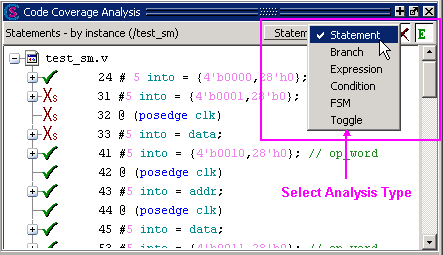
\includegraphics[width=80mm, scale=0.5]{img/v11_questa_code_coverage_analysis.png}
  \caption{Primer \emph{Code Coverage Analysis} prozora}
  \label{fig:questa_code_coverage_analysis}
\end{figure}

Podaci i statitskia se takođe mogu videti u \emph{Object}, \emph{Source} i
\emph{Structure} prozorima.
Što se tiče praćenja funkcionalne pokrivenosti, podaci se mogu analizirati i u
\emph{Covergroups} prozoru (slika \ref{fig:questa_covergroup_window})

\begin{figure}[h!]
  \center
  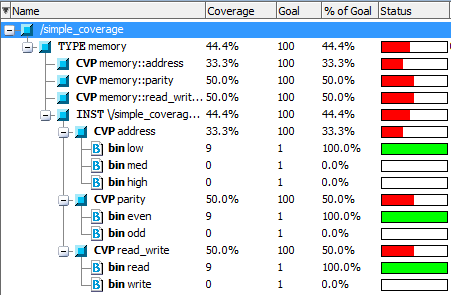
\includegraphics[width=80mm, scale=0.5]{img/v11_simple_coverage.png}
  \caption{Primer \emph{Covergroup} prozora}
  \label{fig:questa_covergroup_window}
\end{figure}

Što se tiče izveštaja o statistici, mogu se generisati u različitim formatima:
tekstualni ili HTML. Mogu sačuvati i sami podaci u UCDB fajlu kako bi se mogli
ponovo učitati ili spajati sa podacima iz prethodnih simulacija. Ovaj korak se
vrši prilikom regresije o kojoj će biti reči na naredoj vežbi.\\

Generisanje izveštaja se vrši klikom na \emph{Tools \(\rightarrow\) Coverage
  Reports} i odabirom željenog formata. HTML format se često koristi jer daje
dobar vizuelni pregled i željeni podaci se lako pronalaze klikom na odgovarajuće
blokove. Primer je dat na slici \ref{fig:questa_coverage_report}.

\begin{figure}[h!]
  \center
  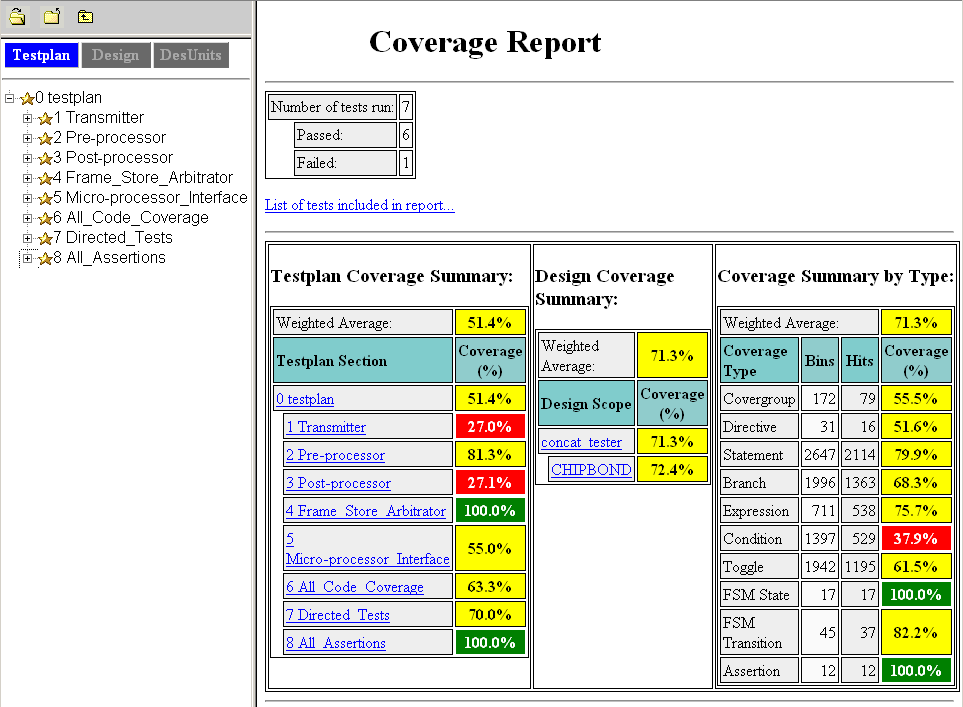
\includegraphics[width=\textwidth]{img/v11_questa_coverage_report.png}
  \caption{Primer izveštaja}
  \label{fig:questa_coverage_report}
\end{figure}

%========================================================================================
% Section
%========================================================================================

\section{Zadaci}

\paragraph{Zadatak}

Za primer modula datog na početku vežbe i u dodatnim materijalima sakupiti
podatke o pokrivenosti koji se odnose na sledeći uslov u verifikacionom planu:
``Na \emph{data} signalu će se pojaviti granične vrednosti (0 i 255)''.
Definisati \emph{bin}-ove za ove dve vrednosti, kao i jedan \emph{bin} za sve
preostale vrednosti.

\paragraph{Zadatak}

Proširiti prethodni zadatak tako da pokrije i sledeći zahtev: ``Operacije upisa
i čitanja (\emph{rw} signal) treba da budu obavljene sa obe vrednosti parnosti
(\emph{par} signal)''.

\paragraph{Zadatak}

Proširiti prethodni zadatak tako da pokrije i sledeći zahtev: ``Potrebno je
upisati granične vrednosti podataka (0 i 255) na granične adrese (0 i 255)''.

\paragraph{Zadatak}

Proširiti prethodni zadatak tako da pokrije i sledeći zahtev: ``Pratiti
vrednosti pročitanih podataka, pri čemu podaci sa \emph{par}=1 nisu od
interesa''.

%========================================================================================

